\documentclass[12pt,a4paper]{article}
\usepackage[utf8]{inputenc}
\usepackage[T1]{fontenc}
\usepackage[english]{babel}
\usepackage{csquotes} 
\usepackage[]{mcode}
\usepackage[left=0.3cm,right=0.7cm,top=1.6cm,bottom=1.6cm]{geometry}
\geometry{bindingoffset=1.5cm}
\usepackage{graphicx}
\usepackage[section]{placeins}
\usepackage[parfill]{parskip}
\usepackage{fancyhdr}
\setlength{\headheight}{15.2pt}
\pagestyle{fancy}
\lhead{}
\chead{\textit{ \nouppercase{\leftmark}}}
\rhead{}
\usepackage{hyperref}

\begin{document}	
	
	\title{Anisotropic diffusion for denoising and edge detection}
	\author{Simon \textsc{Lebastard}}
	\date{January, 7th, 2016}
	
\maketitle
	
\section{General principles}

\subsection{Space-scales}
A picture can have a range of different important scales. It can bear information at a low spatial frequency, while details will be held in the high frequencies of the picture.\\
When receiving a damaged picture, we might not be able to know what the most important "spectral scale" for the image is. Below is an exemple of a space-scale of a 1D signal (source: Perona \& Malik)
\\
From an image we received, we basically want to produce a wide range of scale space, so that if the image was damaged during transmission, information from different frequencies can be recovered.
\\
\begin{figure}[h]
	\centering
	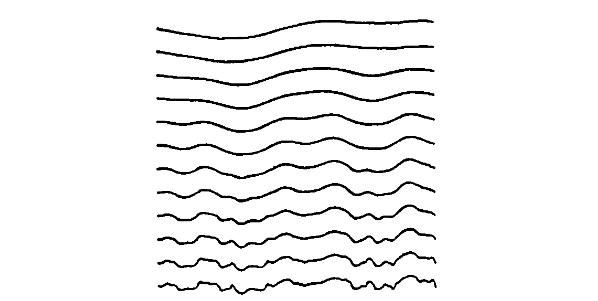
\includegraphics[scale=0.3]{ScaleSpace_Example.png}
	\caption{Scale space of a 1D signal. Source: Perona \& Malik}
\end{figure}

\subsection{Isotropic diffusion}

Convoluting with Gaussian kernels of increasing width is comparable to solving the diffusion problem, which general equation is:

\begin{equation}
I_{t} = div(c(x,y,t) \nabla I)
\end{equation}

In isotropic situation $c(x,y,t)$ is only a function of time, and in the case of a time-constant environment \textbf{$c$ is a constant}.
The solution of this equation in this case is the following:
\begin{equation}
I(x,y,t)=\frac{1}{\sqrt{4 \pi c t}}\int_{ }^{ } I(x',y',0)\exp^{-\frac{(x-x')^{2} + (y-y')^{2}}{4ct}}dx'dy'
\end{equation}
The solution can be interpreted as the convolution of the original image with the gaussian kernel:
\begin{equation}
G(x,y,t)=\frac{1}{\sqrt{4 \pi c t}}\exp^{-\frac{x^{2} + y^{2}}{4ct}}
\end{equation}
the deviation of which increases linearly with time, and is a linear function of $c$.
This result suits the intuition that the gaussian kernel expands wih time, leading to fading high frequences.


To illustrate the different kinds of solutions I'll use the following picture of Venise. First here the result of isotropic diffusion for different kernel width.
\begin{figure}[h]
	\centering
	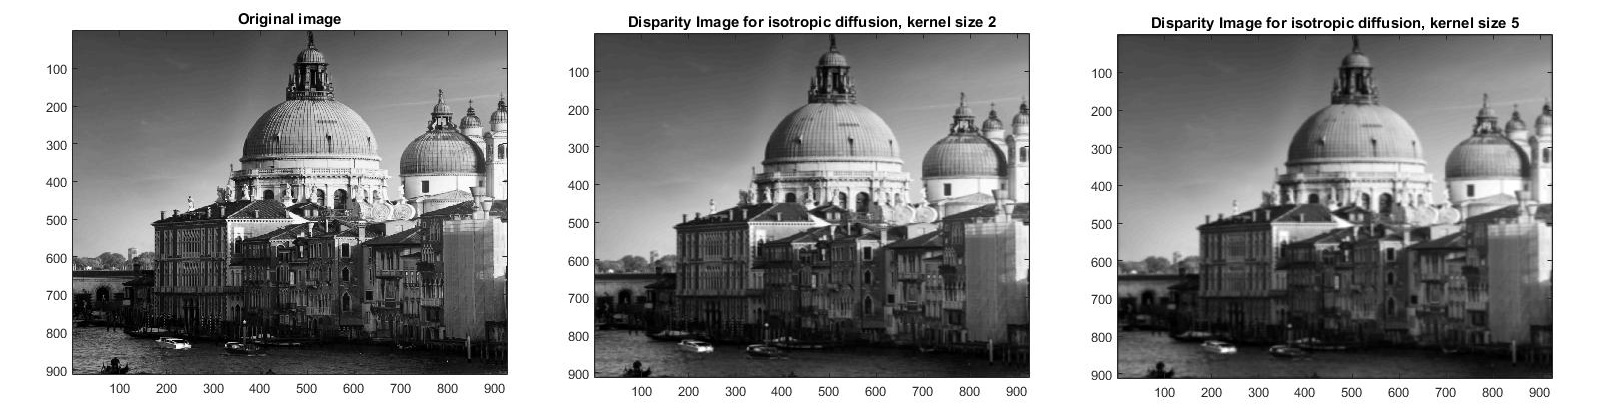
\includegraphics[scale=0.6]{isotropic_diffusion.jpg}
	\caption{The result of isotropic diffusion for a constant c = 1, for various kernel width}
\end{figure}
Those results were computed in the exact same manner that was tought during class. You can download the Matlab code as well as the image ressources from:
\url{https://github.com/slebastard/TIVA\_anisotropic\_diffusion}

Gaussian convolution can generate a scale space that have some fine properties. However it also has some pretty obvious drawbacks, some of which are:
\begin{itemize}
	\item Noise disappears but so do edges. The high peaks of the gradients tend to smoothen.
	\item Edges are naturally shifted away from their true location when the image is convoluted with an increasingly flat Gaussian kernel. That means that even if we recognize an edge in a coarse scale image, we won't be able to figure out the true position of that edge so easily.
\end{itemize}

Note that the Laplacian of Gaussian (LoG) is often used for the isotropic diffusion methods. It simply is the difference between two or more gaussian kernels of different width, and presents two advantages: it is linear, and it seems to be very close from the way mammals see.

\section{Anisotropic diffusion and the Perona \& Malik study}

In the general case the diffusion factor $c(x,y,t)$ is a function of space and time.
An ideal case would be if we could make it to set $c=0$ on the edges of the objects and $c \neq 0$ otherwise. There would then be a blurring inside each regions, without the regions being mixed up.

For some cases of diffusion factors, taken as functions of $|| \nabla I ||$, the edges of the image will be preserved, they will even seem enhanced (though they technically will not be).

Perona \& Malik worked on a specific range of solutions, generated from two classes of diffusion factors:
\begin{equation}
	c_{\kappa}(||\nabla I||) = \exp((-\frac{||\nabla I||}{\kappa})^{2})
\end{equation}
and
\begin{equation}
c_{\kappa}(||\nabla I||) = \frac{1}{1+(\frac{|| \nabla I ||}{\kappa})^{2}}
\end{equation}

In both cases we can see that the spots with a high gradient will generate a low diffusion factor, which means that diffusion will not occur much around the edges. Those two diffusion functions result from a compromise between blurring the low (intensity) variations spots while preserving the edges.

Note that the $\kappa$ parameter plays an important role: when high, only very important gradients will induce a low diffusion factor. That means that the asymptotic situation $\kappa \to \infty$ is equivalent to isotropic diffusion, while a very low value for $\kappa$ will mean that spots with a fairly high gradient (edges, that is) will be spared from diffusion.

From this anisotropic diffusion we can generate anisotropic scale space that have good properties.

As can be seen in the results (page 4), the low-resolution image that was generated through anisotropic diffusion make it to preserve the most important edges for a sufficiently low $\kappa$ value. The major gradients in the image are preserved, they even appear enhanced because of the variation of local contrasts around an edge.

\section{Applications}

\subsection{Anisotropic filters for denoising and edge detection}

Anisotropic diffusion is an effective process for denoising (through blurring) while preserving the edges (which cannot be done with a mere gaussian kernel convolution). 

Is was shown before that building a space scale with an isotropic diffusion would lead to blurring the edges, which is a problem as what we seek to do is to represent all the objects of different scales in the image without alterring them, which implies that we must be able to detect edges of all objects in the image from the scale space.
Edges detection can be made easy by running the diffusion process backwards. But the problem is ill-posed and mostly leads to unstable solution.

Anisotropic diffusion with just the right diffusion factor, as a function of $|| \nabla I||$ can lead to similar results while going forward in time (thus preventing us from any unstability issue).

In their paper, Perona \& Malik compared the result of anisotropic diffusion with the canny detector in terms of edges enhancement. $|| \nabla I ||$ is compared for the two methods.

\subsection{Thermal conduction in 'anisotropic' environment}

There are several exemples of situations of anisotropic (in the sense that was defined earlier, which in physics is equivalent to the term 'inhomogeneous') diffusion:
Diffusion in a porous environement, and more generally in inhomogeneous environement, where the diffusion constant $c(x,y,t)$ will depend on the layer, material or physical state that is at position $(x,y)$ at time $t$. In fact we have
	\begin{equation}
	c = \frac{k}{\rho C_{V}}
	\end{equation}
	where $\rho$ is the material density, $k$ is its thermal conductivity, $C_{V}$ its specific heat.
	Upon hypothesis a resolution scheme similar to the one explained below, for the right diffusion function, could be used.

\subsection{Bilateral filter}

Instictively, anisotropic diffusion is closed to bilateral filtering, because a pixel in the picture is replaced by the average of neighboors only if the neightboors have similar intensity levels. That's why edges are preserved here: the white-grey of the sky won't be taken into consideration in the black of the root next to the edges, because the diffusion factor on the edge of the roof is low enough.
\\
Indeed the discrete anisotropic propagation formula described in the how-to below is exactly equivalent to:
\begin{equation}
\frac{\partial I_{r}}{\partial t} = A \sum_{s \in N(r)}c(I_{s} - I_{r})(I_{s} - I_{r})
\end{equation}
which is precisely a gradient descent algorithm step, with A an exploration speed factor and for the following local energy function:
\begin{equation}
E(I_{r}) = \sum_{s \in N(r)}c(I_{s} - I_{r})(I_{s} - I_{r}) = \sum_{s \in N(r)}V(I_{s}, I_{r})
\end{equation}

where $V(I_{s}, I_{r}) = V(I_{s} - I_{r})$ is an increasing function of the distance between $I_{s}$ and $I_{r}$. In this way the solution from the anisotropic discrete scheme computes a mean value from direct neighboors the value of which is similar. This process is done by minimizing an energy functionnal, whereas bilateral filters use gaussian convolutions, but the two schemes are very much alike. One difference is that gaussian convolution directly computes a mean value over a wide range of geometrical neighboors, while anisotropic diffusion computes a mean value implicitely, and the process is only tangible for a big number of time loops. 

\begin{figure}[h]
	\centering
	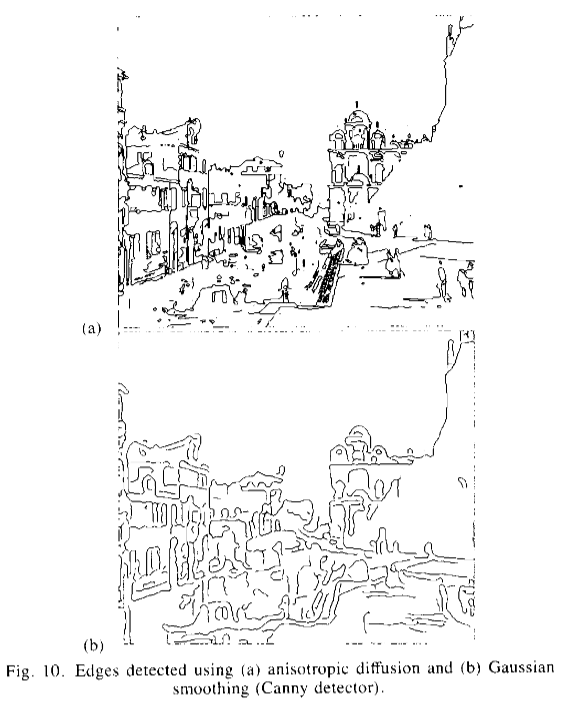
\includegraphics[scale=0.5]{EdgeEnhancement_Example.png}
	\caption{The results of anisotropic diffusion (a) and canny detection (b) on the intensity gradient map ($||\nabla I||$). Source: Perona \& Malik}	
\end{figure}

\section{Anisotropic filters: how to}

\subsection{Computing the filter}

To perform an anisotropic filter, the modifications in the image from one step to the next are controlled by discretizing the general diffusion equation into:
\begin{equation}
I_{i,j}^{t+1} = I_{i,j}^{t} + \lambda * (c_{N} \nabla_{N}I + c_{S} \nabla_{S}I + c_{W} \nabla_{W}I + c_{E} \nabla_{E}I)
\end{equation}
according to the method from Perona \& Malik,
where $\nabla_{N}I$ will here mean the finite-difference:
\begin{equation}
\nabla_{N}I_{i,j} = I_{i-1,j} - I_{i,j}
\end{equation} , and $c_{N}$ is the diffusion factor for the northern direction from this pixel: 
\begin{equation}
c_{N,i,j}^{t} = g((||\nabla I||)_{i+\frac{1}{2},j}^{t})
\end{equation}
Here g would be one of the two functions that Perona \& Malik used in for their works.
\\
Then we would only have to run a script that, from the original image, computes the blurred image. This is what it looks like for a single time loop.
\begin{lstlisting}
[w,h] = size(img);
actualized_img = zeros(size(img));

for ab = 1:w
	for or = 1:h
		dif_coef = compute_coef(img, ab, or, kappa);
		fin_diff = compute_difference(img, ab, or);
		actualized_img(ab,or) = img(ab,or) + lambda*dot(dif_coef, fin_diff);
	end
end
\end{lstlisting}
Here the compute\_coef function returns the value of the diffusion factors around $(ab,or)$, using the quadratic or exponential function with the parameter $\kappa$.
The compute\_difference function evaluates the finite-differences of intensity around $(ab,or)$.

\subsection{Results}

Here are the results from my program, computed for different $\kappa$ values at a given $\lambda=0.25$. Results also show the influence of diffusion time at a given $\kappa$.

\begin{figure}[h]
	\centering
	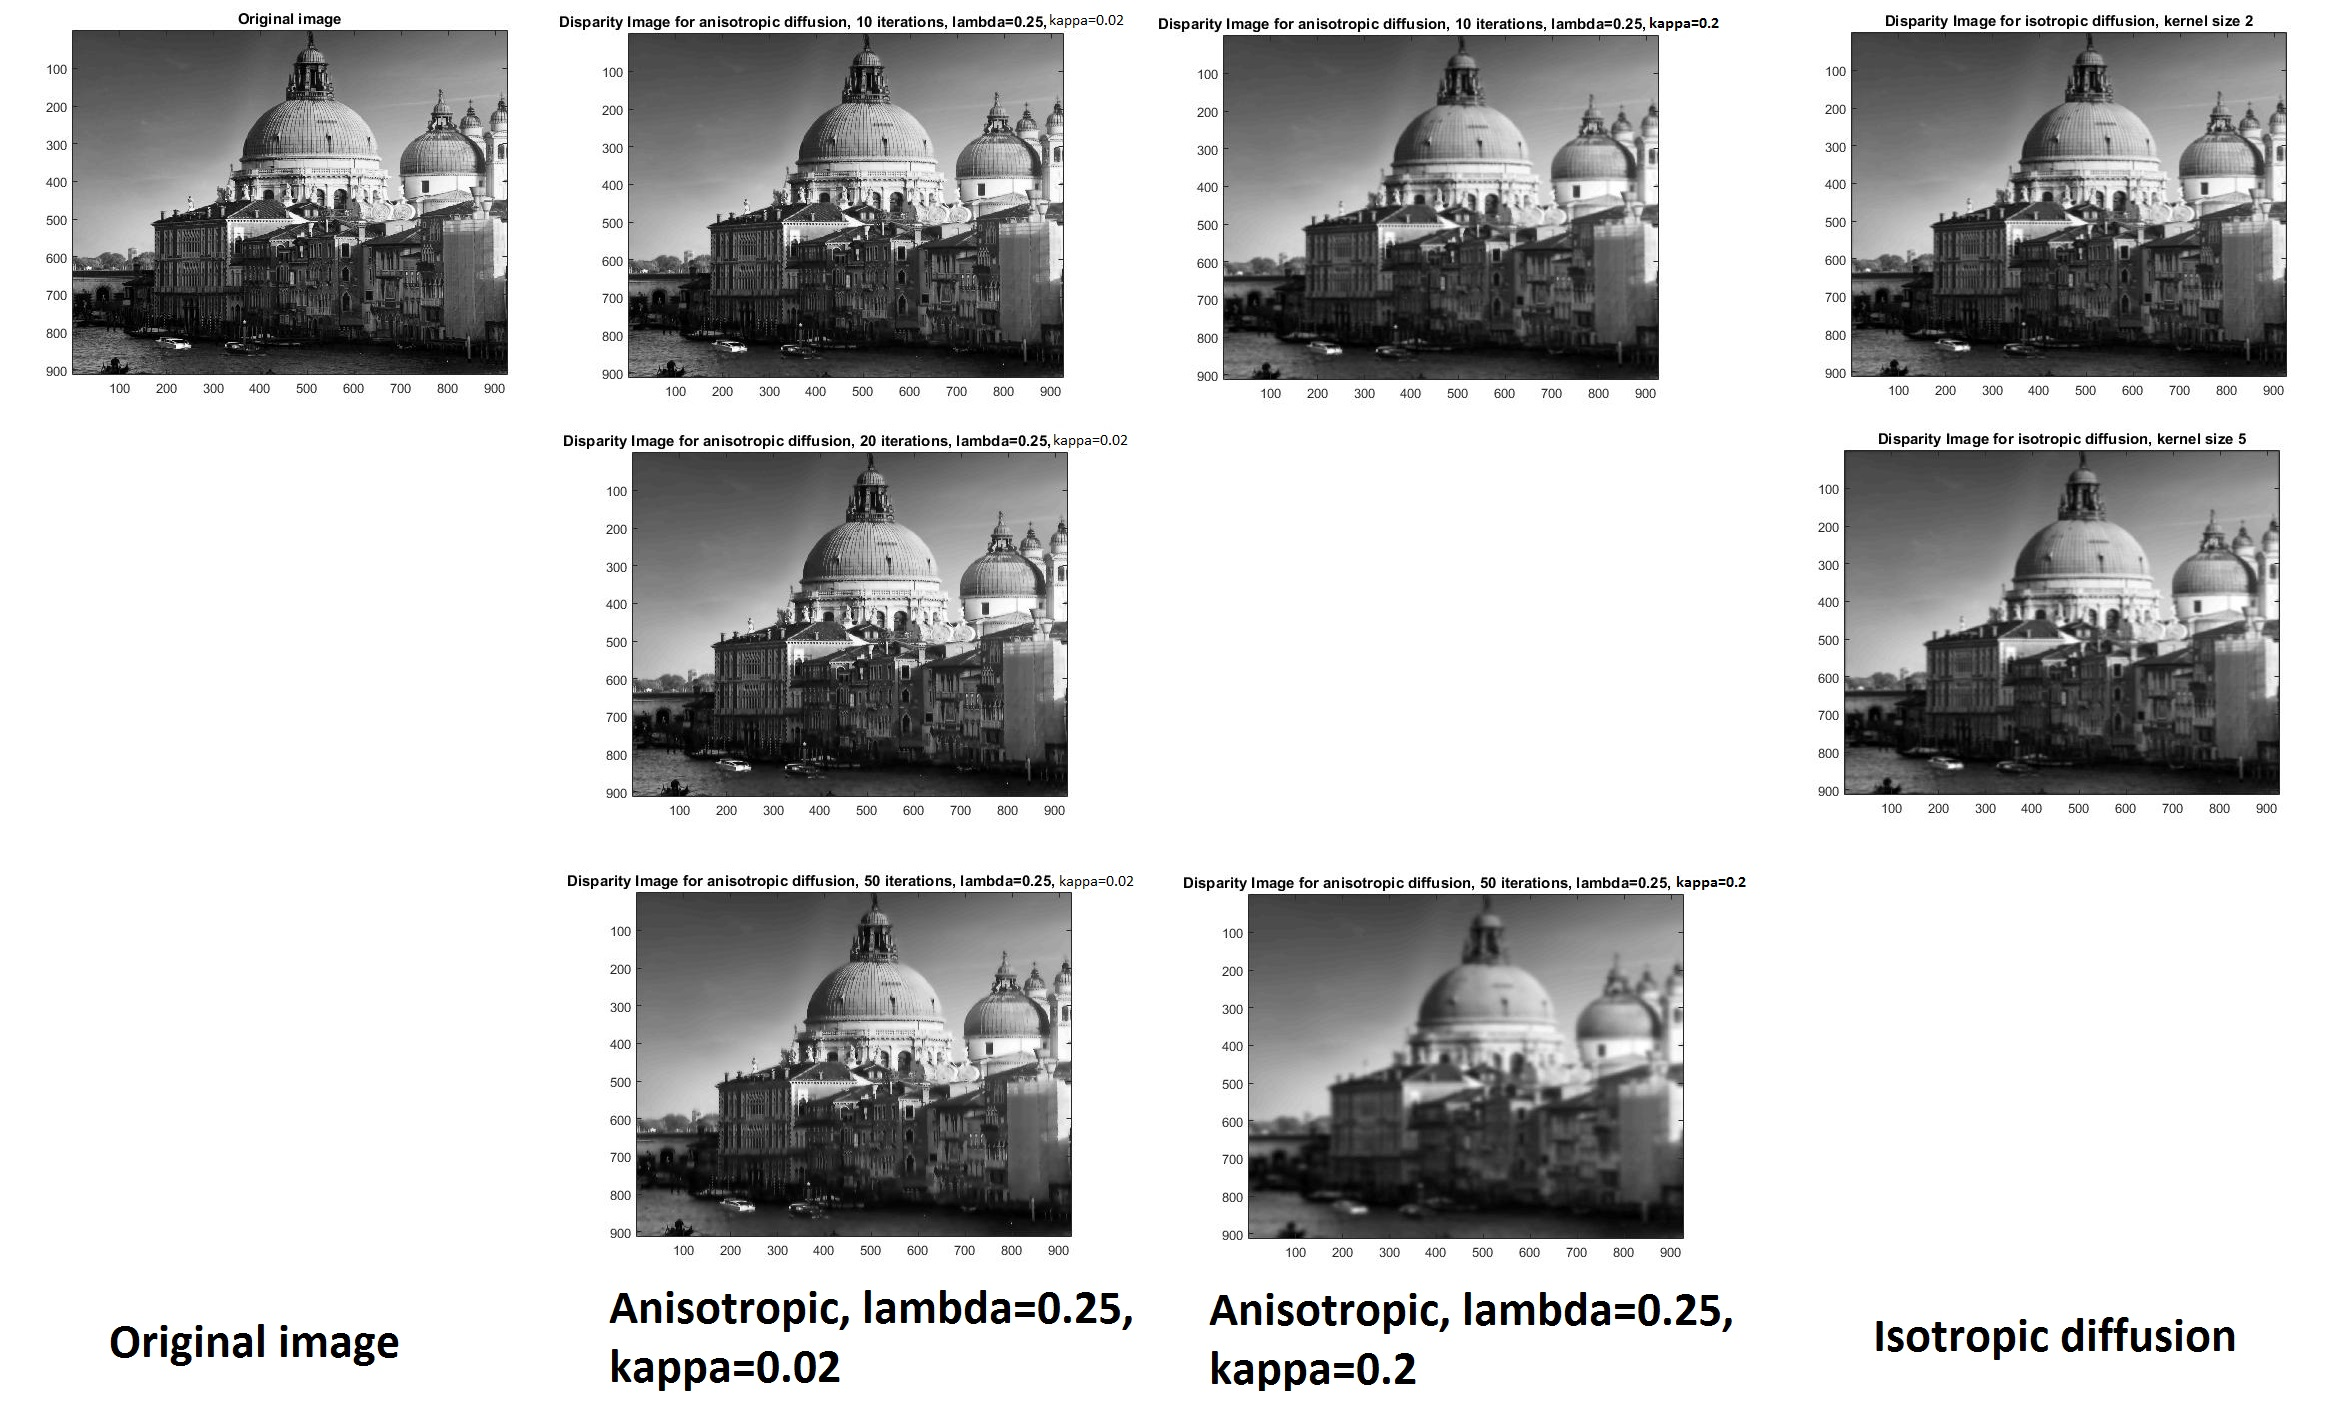
\includegraphics[scale=0.42]{anisotropic_diffusion.jpg}
	\caption{Results from the Matlab script for anisotropic diffusion, for different $\kappa$ values and number of iterations}	
\end{figure}

Once again you can checkout the code as well as the solutions and ressources used at: \url{https://github.com/slebastard/TIVA\_anisotropic\_diffusion}

As most differential problems, this can also be resolved by minimizing an image functionnal. This is not the approach that has been dealt with here.

\section{Bibliography}
\begin{itemize}
	\item \url{http://image.diku.dk/imagecanon/material/PeronaMalik1990.pdf}\\
	Title: Scale-space and edge detection using anisotropic diffusion\\
	Authors: Perona \& Malik\\
	July 1990
	\item \url{http://www.cs.utah.edu/~manasi/coursework/cs7960/p2/project2.html}\\
	Project title: Anisotropic diffusion\\
	Author: M. Datar
	\item \url{http://www.mia.uni-saarland.de/weickert/Papers/book.pdf}\\
	Title: Anisotropic diffusion in image processing\\
	Author: J. Weickert
	At: B.G. Teubner Stuttgart
	\item \url{http://www.sciencedirect.com/science/article/pii/0011227579900547}\\
	Title: Model calculations on heat flow in inhomogeneous thermal systems\\
	Authors: A.W Pattulo \& J.C.A van der Sluijs
\end{itemize}


\end{document}